\appendix
\renewcommand\thechapter{\Alph{chapter}}

\chapter{Lemma on Bounded Solutions}
\label{appendix:lemma-on-bounded-solutions}

\begin{lemma*}[On bounded solutions]
	Let $f(t, z)$ be defined for $t \ge t_0$, $|z| < +\infty$,
	Let $f(t, z)$ be a function that is continuous with respect to $t$, continuously differentiable with respect to $z$, and has the following properties:
	\begin{itemize}
		\item[(i)] for $|z| < \rho$, $\rho > 0$, the estimate $|f(t, z)| < \eta_{\rho}(t)|z|$ is valid, where $\eta_{\rho}(t) \in L_1(t_0; +\infty)$;
		\item[(ii)] for all $z_1$, $z_2$ such that $|z_{1,2}| < \rho$, $\rho > 0$, there exists a function $\tilde{\eta}_{\rho}(t) \in L_1(t_0; +\infty)$, such that $|f(t, z_2) - f(t, z_1)| \le \tilde{\eta}_{\rho}(t) |z_2 - z_1|$;
		\item[(iii)] for $|z| < \rho$, $\rho > 0$, the estimate $|f_z(t, z)| < \theta_{\rho}(t) |z|$ is valid, where $\theta_{\rho} \in L_1(t_0, +\infty)$;
		\item[(iv)] for all $z_1$, $z_2$ such that $z_{1,2} < \rho$, $\rho > 0$, there exists function $\tilde{\theta}_{\rho} \in L_1(t_0; +\infty)$, such that $|f_z(t, z_2) - f_z(t, z_1)| \le \tilde{\theta}_{\rho} |z_2 - z_1|$.
	\end{itemize}
	Then for the equation
	\begin{equation}
		z_{tt} - \alpha z_t + f(t, z) = 0, \quad \alpha > 0
		\label{eq:lemma-bs-main}
	\end{equation}
	the following statements are valid:
	\begin{itemize}
		\item[(A)] for each solution $z(t)$ of equation \eqref{eq:lemma-bs-main} that is bounded when $t \to +\infty$ there exists $C \in \mathbb{R}$ such that $z(t) \to C$ as $t \to +\infty$;
		\item[(B)] for each $C \in \mathbb{R}$ there exists unique solution $Z(t, C)$ of equation \eqref{eq:lemma-bs-main}, defined on a segment $(t_C; +\infty)$, such that
		\begin{equation}
			Z(t, C) = C + o(1), \quad t \to +\infty;
		\end{equation}
		\item[(C)] family of solutions $Z(t, C)$ is $C^1$-smooth with respect to the parameter $C$.
	\end{itemize}
\end{lemma*}
\begin{proof}
	Let us prove the statement (A) first.
	Applying the method of variation of parameters one can find that a solution of equation \eqref{eq:lemma-bs-main} satisfies the equality:
	\begin{equation}
		z(t) = \varkappa_1 + \varkappa_2 e^{\alpha t} + \int \limits_{t_0}^{t} e^{\alpha \eta} \left( \int \limits_{\eta}^{+\infty} e^{-\alpha \xi} f(\xi, z(\xi)) d\xi \right) d\eta.
	\end{equation}
	It follows from the condition (i) that if $z(t)$ is bounded while $t \to +\infty$ then the integral
	\begin{equation}
		\int \limits_{t_0}^{+\infty} e^{\alpha \eta} \left( \int \limits_{\eta}^{+\infty} e^{-\alpha \xi} f(\xi, z(\xi)) d\xi \right) d\eta
	\end{equation}
	converges.
	Furthermore for all bounded solutions $\varkappa_2 = 0$, hence $z(t)$ tends to some constant for $t \to +\infty$.
	That proves the point (A).
	
	Move on to the point (B).
	We make the change of variable $u(t) = z(t) - C$, where $C$ is arbitrary constant.
	Rewrite equation \eqref{eq:lemma-bs-main} in the form of system of equations
	\begin{equation}
		y_t = Ay + F(t, y),
		\label{eq:lemma-bs-system}	
	\end{equation}
	where
	\begin{equation*}
		y = \begin{pmatrix}
			u \\ v
		\end{pmatrix}, \quad
		A = \begin{pmatrix}
			0 & 1 \\
			0 & \alpha
		\end{pmatrix}, \quad
		F(t, y) = \begin{pmatrix}
			0 \\ f(t, u + C)
		\end{pmatrix}.
	\end{equation*}
	Now we apply Theorem 9.1 from \cite[Chapter XII]{Hartman} to system \eqref{eq:lemma-bs-system}.
	It states that \eqref{eq:lemma-bs-system} {\it has a solution which tends to zero at infinity} \underline{if} the following conditions are satisfied:
	\begin{itemize}
		\item[(1)] function $F(t, y)$ is continuous and $||F(t, y)|| \le \lambda(t)$ for $t \in [t_0; +\infty)$, $||y|| \le \rho$, where $\lambda(t) \in L_1(t_0; +\infty)$;
		\item[(2)] for all $g(t) = col(g_1(t), g_2(t))$, $g(t) \in L_1(t_0; +\infty)$ there exists a solution $y(t) \in L_0^{\infty}(t_0; +\infty)$ of the inhomogeneous system
		\begin{equation}
			y_t = Ay + g(t);
			\label{eq:lemma-bs-hartman}
		\end{equation}
		(hereinafter by $||\cdot||$ we denote the Euclidean norm in $\mathbb{R}$).
	\end{itemize}
	
	Firstly, due to condition (i) if $|u| \le \rho$ and $t > t_0$ relation $||f(t, u, C)|| \le \rho \eta_{\rho} (t)$ takes place, moreover $\eta_{\rho}(t) \in L_1(t_0; +\infty)$, hence the condition (1) of the above-mentioned theorem is satisfied.
	Secondly, general solution of the inhomogeneous system of equations \eqref{eq:lemma-bs-hartman} can be written as:
	\begin{eqnarray}
		&& u(t) = C_2 + \int \limits_{t_0}^{t} \left( g_1(\eta) + e^{\alpha \eta} \left( C_1 - \int \limits_{+\infty}^{\eta} e^{-\alpha \xi} g_2(\xi) d\xi \right) \right) d\eta; \\
		&& v(t) = u_t(t) - g_1(t).
	\end{eqnarray}
	Since $g_{1,2}(t) \in L_1(t_0; +\infty)$ one can choose appropriate parameters $C_1$, $C_2$ in order to get a solution which tends to zero while $t \to +\infty$, so the condition (2) of the theorem is also met.
	Thereby both of the conditions for the applied theorem take place for the system \eqref{eq:lemma-bs-system}.
	That implies existence of a solution $z(t)$ of \eqref{eq:lemma-bs-main} that approaches a given constant $C$ while $t \to +\infty$ for all $C$.
	
	Now we prove the uniqueness of such solution.
	Suppose that for the same $C$ there exist two solutions $u_{1,2}(t)$ for equation
	\begin{equation}
		u_{tt} - \alpha u_t + f(t, u + C) = 0.
		\label{eq:lemma-bs-u}
	\end{equation}
	Consider their difference $\Delta(t) = u_2(t) - u_1(t)$.
	It satisfies the equation
	\begin{equation}
		\Delta_{tt} - \alpha \Delta_t + R(t) \Delta = 0,
		\label{eq:lemma-bs-difference}
	\end{equation}
	and a boundary condition $\Delta \to 0$ as $t \to +\infty$.
	Here
	\begin{equation}
		R(t) \equiv \dfrac{f(t, u_2(t) +C) - f(t, u_1(t) + C}{u_2(t) - u_1(t)}.
	\end{equation}
	Due to condition (ii) we can apply Theorem 11 from \cite[Chapter 3]{Coppel}.
	It states that there exists a homeomorphism between the bounded solutions of the equation \eqref{eq:lemma-bs-difference} and solutions of equation
	\begin{equation}
		\Delta_{tt} - \alpha \Delta_t = 0,
	\end{equation}
	moreover (see a note to that theorem in \cite{Coppel}) this homeomorphism is a linear map.
	It means that only a zero solution of \eqref{eq:lemma-bs-difference} satisfies the zero asymptotic at infinity, i.e. $u_2(t) \equiv u_1(t)$.
	Thus we have proved the existence of the family of solutions $Z(t, C)$ parametrised by $C \in \mathbb{R}$.
	Statement (B) is proved.
	
	To prove the statement (C) one can note that the derivative
	\begin{equation}
		\dfrac{\partial Z}{\partial C}(t, C) \equiv \Theta(t, C)
	\end{equation}
	satisfies the equation \eqref{eq:lemma-bs-u} after differentiation with respect to $C$, moreover $\Theta(t, C) \to 0$ as $t \to +\infty$.
	We have
	\begin{equation}
		\Theta_{tt} - \alpha \Theta_t + f_z(t, u + C) \Theta + f_z(t, u + C) = 0.
	\end{equation}
	Here we can use Theorem 11 from \cite[Chapter 3]{Coppel} again, and using the condition (iii) we can conclude that there exists a solution of this equation $\Theta(t, C)$ such that $\Theta(t, C) \to 0$ as $t \to +\infty$, and function $\Theta(t, C)$ is continuous with respect to the parameter $C$.
	That completes the proof of lemma.
\end{proof}

\chapter{Solutions of Duffing equations}
\label{appendix:solutions-of-duffing-equations}

\chapter{Strips Mapping Theorems}
\label{appendix:strips-mapping-theorems}

% TODO: Read through this carefully.
\begin{theorem}[On h-strips mapping]
\label{thm:h-strips-mapping}
	Let Poincar\'e map $\mathcal{P}$ and its inverse $\mathcal{P}^{-1}$ be defined on a complete (see Definition~\ref{def:complete-island-set}) island set $\bigcup_{i \in S} D_i$, where $S$ is a finite or countable set of indices.
	Let for all $i, j \in S$ the set $V_{ij} = \mathcal{P}^{-1} (D_j) \cap D_i$ is non-empty, $\mathcal{P}$ is defined on a
	 closure $\overline{V_{ij}}$, and one of the following two conditions holds:
	\begin{enumerate}
		\item[(1)] the borders $\alpha_i^{\pm}$ of an island $D_i$ are increasing curves, $\forall \vb{p} \in \overline{V_{ij}}$ the signs of $\{ a_{mn} \}$ in the matrix of the linear operator $D \mathcal{P}_{\vb{p}} = (a_{mn})$ have exactly one of the following configurations\footnote{By ``$+$'' and ``$-$'' sign we mean \underline{strict} inequalities $a_{mn} > 0$, $a_{mn} < 0$ to be held.}:
			\begin{center}
				(a) $\begin{psm} + & + \\ + & + \end{psm}$, \quad
				(b) $\begin{psm} - & - \\ - & - \end{psm}$, \quad
				(c) $\begin{psm} + & + \\ - & - \end{psm}$, \quad
				(d) $\begin{psm} - & - \\ + & + \end{psm}$;
			\end{center}
			and at the same time the borders $\alpha_j^{\pm}$ of $D_j$ are increasing curves for cases (a), (b), and decreasing curves for (c), (d);
		\item[(2)] the borders $\alpha_i^{\pm}$ of an island $D_i$ are decreasing curves, $\forall \vb{p} \in \overline{V_{ij}}$ signs of $\{ a_{mn} \}$ in the matrix of the linear operator $D \mathcal{P}_{\vb{p}} = (a_{mn})$ have exactly one of the following configurations:
			\begin{center}
				(a) $\begin{psm} + & - \\ - & + \end{psm}$, \quad
				(b) $\begin{psm} - & + \\ + & - \end{psm}$,	\quad
				(c) $\begin{psm} + & - \\ + & - \end{psm}$, \quad
				(d) $\begin{psm} - & + \\ - & + \end{psm}$;		
			\end{center}
			and at the same time borders $\alpha_j^{\pm}$ of $D_j$ are decreasing curves for cases (a), (b), and increasing for (c), (d);
	\end{enumerate}
	and moreover $\exists \mu > 1$ such that $\forall p \in \overline{V_{ij}}$, $|a_{11}| \ge \mu$.
	Then
	\begin{itemize}
		\item[(i)] for any \emph{h}-strip $H \in D_i$, $\mathcal{P} (H) \cap D_j = \widetilde{H}_j$ is also an \emph{h}-strip;
		\item[(ii)] $d_{\mathrm{h}}(\widetilde{H}_j) \le (1 / \mu) d_{\mathrm{h}}(H)$ (here $d_{\mathrm{h}}(\cdot)$ is an \emph{h}-strip thickness in a sence of Definition~\ref{def:h-thickness}).
	\end{itemize}
\end{theorem}
\begin{proof}
	Let's fix indices $i, j$ and prove the theorem for a pair of islands $D_i$, $D_j$.
	Consider the case (1а), other cases can be treated in an analogous way.
	Denote by $\mathbf{e}_1$, $\mathbf{e}_2$ the vectors
	\begin{equation}
		\mathbf{e}_1 = \begin{pmatrix} 1 \\ 0 \end{pmatrix}; \quad \mathbf{e}_2 = \begin{pmatrix} 0 \\ 1 \end{pmatrix}.
	\end{equation}
	Define the following set of {\it cones}:
	\begin{align*}
		\mathbb{R}_{++}^2 = \{ \mathbf{v} \, | \, \mathbf{v} = x \mathbf{e}_1 + y \mathbf{e}_2, \; x > 0, y > 0 \}; \\
		\overline{\mathbb{R}}_{++}^2 = \{ \mathbf{v} \, | \, \mathbf{v} = x \mathbf{e}_1 + y \mathbf{e}_2, \; x \ge 0, y \ge 0 \}; \\
		\mathbb{R}_{+-}^2 = \{ \mathbf{v} \, | \, \mathbf{v} = x \mathbf{e}_1 + y \mathbf{e}_2, \; x > 0, y < 0 \}; \\
		\overline{\mathbb{R}}_{+-}^2 = \{ \mathbf{v} \, | \, \mathbf{v} = x \mathbf{e}_1 + y \mathbf{e}_2, \; x \ge 0, y \le 0 \}; \\
		\mathbb{R}_{-+}^2 = \{ \mathbf{v} \, | \, \mathbf{v} = x \mathbf{e}_1 + y \mathbf{e}_2, \; x < 0, y > 0 \}; \\
		\overline{\mathbb{R}}_{-+}^2 = \{ \mathbf{v} \, | \, \mathbf{v} = x \mathbf{e}_1 + y \mathbf{e}_2, \; x \le 0, y \ge 0 \}; \\
		\mathbb{R}_{--}^2 = \{ \mathbf{v} \, | \, \mathbf{v} = x \mathbf{e}_1 + y \mathbf{e}_2, \; x < 0, y < 0 \}; \\
		\overline{\mathbb{R}}_{--}^2 = \{ \mathbf{v} \, | \, \mathbf{v} = x \mathbf{e}_1 + y \mathbf{e}_2, \; x \le 0, y \le 0 \}.
	\end{align*}
	As the \underline{first} step of the proof, we show that the signs of entries of the matrix of linear operator $D \mathcal{P}_{\vb{p}} = ( a_{mn} )$ uniquely determine the mapping of the cones in each point $\vb{p}$ of the set $\overline{V_{ij}}$.
	For the case (a) we have:
	\begin{equation*}
	\forall \mathbf{v} = \begin{pmatrix} x \\ y \end{pmatrix} \in \overline{\mathbb{R}}_{++}^2, \ D \mathcal{P}_{\vb{p}}(\mathbf{v}) = \begin{pmatrix} a_{11} & a_{12} \\ a_{21} & a_{22} \end{pmatrix} \begin{pmatrix} x \\ y \end{pmatrix} = \begin{pmatrix} \widetilde{x} > 0 \\ \widetilde{y} > 0\end{pmatrix} \in \mathbb{R}_{++}^2.	
	\end{equation*}
	It is easy to check that in the case (1) $D \mathcal{P}_{\vb{p}}$ maps the cones as follows:
	\begin{eqnarray*}
		(\textup{a}) & D \mathcal{P}_{\vb{p}} (\overline{\mathbb{R}}_{++}^2) \in \mathbb{R}_{++}^2, \quad D \mathcal{P}_{\vb{p}} (\overline{\mathbb{R}}_{--}^2) \in \mathbb{R}_{--}^2; \\
		(\textup{b}) & D \mathcal{P}_{\vb{p}} (\overline{\mathbb{R}}_{++}^2) \in \mathbb{R}_{--}^2, \quad D \mathcal{P}_{\vb{p}} (\overline{\mathbb{R}}_{--}^2) \in \mathbb{R}_{++}^2; \\
		(\textup{c}) & D \mathcal{P}_{\vb{p}} (\overline{\mathbb{R}}_{++}^2) \in \mathbb{R}_{+-}^2, \quad D \mathcal{P}_{\vb{p}} (\overline{\mathbb{R}}_{--}^2) \in \mathbb{R}_{-+}^2; \\
		(\textup{d}) & D \mathcal{P}_{\vb{p}} (\overline{\mathbb{R}}_{++}^2) \in \mathbb{R}_{-+}^2, \quad D \mathcal{P}_{\vb{p}} (\overline{\mathbb{R}}_{--}^2) \in \mathbb{R}_{+-}^2.
	\end{eqnarray*}
	In the case (2) one has:
	\begin{eqnarray*}
		(\textup{a}) & D \mathcal{P}_{\vb{p}} (\overline{\mathbb{R}}_{-+}^2) \in \mathbb{R}_{-+}^2, \quad D \mathcal{P}_{\vb{p}} (\overline{\mathbb{R}}_{+-}^2) \in \mathbb{R}_{+-}^2; \\
		(\textup{b}) & D \mathcal{P}_{\vb{p}} (\overline{\mathbb{R}}_{-+}^2) \in \mathbb{R}_{+-}^2, \quad D \mathcal{P}_{\vb{p}} (\overline{\mathbb{R}}_{+-}^2) \in \mathbb{R}_{-+}^2; \\
		(\textup{c}) & D \mathcal{P}_{\vb{p}} (\overline{\mathbb{R}}_{-+}^2) \in \mathbb{R}_{--}^2, \quad D \mathcal{P}_{\vb{p}} (\overline{\mathbb{R}}_{+-}^2) \in \mathbb{R}_{++}^2; \\
		(\textup{d}) & D \mathcal{P}_{\vb{p}} (\overline{\mathbb{R}}_{-+}^2) \in \mathbb{R}_{++}^2, \quad D \mathcal{P}_{\vb{p}} (\overline{\mathbb{R}}_{+-}^2) \in \mathbb{R}_{--}^2.
	\end{eqnarray*}
	
	At a \underline{second} step we show that this mapping preserves Lipschitz and monotonicity properties for curves from $\overline{V_{ij}}$ under $\mathcal{P}$ action.
	Let us show that for the case (1a).
	Note that compactness of $\overline{V_{ij}}$ implies that the supremum exists:
	\begin{equation*}
		\widetilde{\gamma}_{ij} = \sup \dfrac{y}{x}, \ \begin{pmatrix} x \\ y \end{pmatrix} = D \mathcal{P}_{\vb{p}} (\mathbf{v}), \ \vb{p} \in \overline{V_{ij}}, \ \mathbf{v} \in \overline{\mathbb{R}}_{++}^2.
	\end{equation*}
	Further, let $\vb{p}_1, \vb{p}_2 \in \overline{V_{ij}}$, $\vb{p}_1 = (\psi_1, \psi_1')$, $\vb{p}_2 = (\psi_2, \psi_2')$, be two different points such that $\psi_2 \ge \psi_1$, $\psi_2' \ge \psi_2$.
	Let points $\vb{q}_1$, $\vb{q}_2$ be the $\mathcal{P}$-images of the points $\vb{p}_1$, $\vb{p}_2$ correspondingly, $\mathcal{P}(\vb{p}_1) = \vb{q}_1 = (\phi_1, \phi_1')$, $\mathcal{P}(\vb{p}_2) = \vb{q}_2 = (\phi_2, \phi_2')$.
	Let $D \mathcal{P}_{\vb{p}_1}$ be linearization of $\mathcal{P}$ at the point $\vb{p}_1$.
	Then the following expansion is valid:
	\begin{equation}
		\vb{q}_2 = \mathcal{P}(\vb{p}_2) = \vb{q}_1 + D \mathcal{P}_{\vb{p}_1} (\vb{p}_2 - \vb{p}_1) + r(||\vb{p}_2 - \vb{p}_1||),
	\end{equation}
	where $r(||\vb{p}_2 - \vb{p}_1||) / ||\vb{p}_2 - \vb{p}_1|| \to 0$ as $||\vb{p}_2 - \vb{p}_1|| \to 0$ (here $|||\cdot||$ is a Euclidean norm).
	Vector $\vb{p}_{\Delta} = \vb{p}_2 - \vb{p}_1 \in \overline{\mathbb{R}}_{++}^2$, that means that $D \mathcal{P}_{\vb{p}_1} (\mathbf{p}_{\Delta}) = \mathbf{q}_{\Delta} \in \mathbb{R}_{++}^2$, and
	\begin{equation}
		\vb{q}_2 - \vb{q}_1 = \mathbf{q}_{\Delta} + r(||\vb{p}_2 - \vb{p}_1||).
	\end{equation}
	The expression above implies that for ``close enough'' points $\vb{p}_1$, $\vb{p}_2$ their images satisfy the relation $\vb{q}_2 - \vb{q}_1 \in \mathbb{R}_{++}^2$, i.e. $\phi_2 > \phi_1$, $\phi_2' > \phi_1'$.
	Moreover one can choose a value $\gamma_{ij} > \widetilde{\gamma_{ij}}$ such that the following inequality holds:
	\begin{equation}
		0 < \phi_2' - \phi_1' < \gamma_{ij} (\phi_2 - \phi_1).
	\label{eq:ordering}
	\end{equation}
	This ordering is transitive, i.e. \eqref{eq:ordering} and the relation for ``close enough'' point $\vb{p}_2$, $\vb{p}_3$,
	\begin{equation}
		0 < \phi_3' - \phi_2' < \gamma_{ij} (\phi_3 - \phi_2),
	\end{equation}
	imply analogous relation for the points $\vb{p}_1$, $\vb{p}_3$ as well.
	That allows to extend relation \eqref{eq:ordering} over all points $\vb{p}_1, \, \vb{p}_2 \in \overline{V_{ij}}$ that satisfies the conditions $\psi_2 \ge \psi_1$, $\psi_2' \ge \psi_1'$.
	Other cases (1b)-(1d), (2a)-(2d) can be considered in a similar way.
	
	Thus for the case (1) for all points $\vb{p}_1, \, \vb{p}_2 \in \overline{V_{ij}}$, such that $\psi_2 \ge \psi_1$, $\psi_2' \ge \psi_1'$, the coordinates of their $\mathcal{P}$-images $\vb{q}_1 = (\phi_1, \phi_1'), \, \vb{q}_2~=~(\phi_2, \phi_2')$ satisfy one of the following inequalities ($\exists \gamma_{ij}$):
	\begin{subequations}
	\begin{eqnarray}
		(\textup{a}) & 0 < \phi_2' - \phi_1' < \gamma_{ij} (\phi_2 - \phi_1); \label{eq:ordering_1a} \\
		(\textup{b}) & 0 < \phi_1' - \phi_2' < \gamma_{ij} (\phi_1 - \phi_2); \label{eq:ordering_1b} \\
		(\textup{c}) & 0 < \phi_1' - \phi_2' < \gamma_{ij} (\phi_2 - \phi_1); \label{eq:ordering_1c} \\
		(\textup{d}) & 0 < \phi_2' - \phi_1' < \gamma_{ij} (\phi_1 - \phi_2). \label{eq:ordering_1d}
	\end{eqnarray}
	\end{subequations}
	Similarly, for the case (2) for all points $\vb{p}_1, \, \vb{p}_2 \in \overline{V_{ij}}$, such that $\psi_2 \le \psi_1$, $\psi_2' \ge \psi_1'$, the $\mathcal{P}$-images obey one of the following inequalities:
	\begin{subequations}
	\begin{eqnarray}
		(\textup{a}) & 0 < \phi_2' - \phi_1' < \gamma_{ij} (\phi_1 - \phi_2); \label{eq:ordering_2a} \\
		(\textup{b}) & 0 < \phi_1' - \phi_2' < \gamma_{ij} (\phi_2 - \phi_1); \label{eq:ordering_2b} \\
		(\textup{c}) & 0 < \phi_1' - \phi_2' < \gamma_{ij} (\phi_1 - \phi_2); \label{eq:ordering_2c} \\
		(\textup{d}) & 0 < \phi_2' - \phi_1' < \gamma_{ij} (\phi_2 - \phi_1). \label{eq:ordering_2d}
	\end{eqnarray}
	\end{subequations}
	
	As the \underline{third} step we show that for any h-strip $H \in D_i$ its image $\mathcal{P} H \cap D_j = \widetilde{H}_j$ is also an h-strip.
	Let an h-strip $H \in D_i$ be situated between two monotonic h-curves $\widetilde{\alpha}_i^{\pm}$.
	The endpoints of the $\widetilde{\alpha}_i^{\pm}$ belong to the boundaries $\beta_i^{\pm}$ of the island $D_i$, so $H$ is a curvilinear quadrangle bounded by the curves $\widetilde{\alpha}_i^{\pm}$ and segments of the curves $\beta_i^{\pm}$.
	For the case (1a) of the theorem the curves $\widetilde{\alpha}_i^{\pm}$  are increasing.
	Let's consider $\mathcal{P}$-image of the curve $\widetilde{\alpha}_i^+$.
	According to the definition of complete island set $\mathcal{P} (\widetilde{\alpha}_i^+)$ crosses each of the boundaries $\beta_j^{\pm}$ of island $D_j$ at least once.
	At the same time $\mathcal{P} (\widetilde{\alpha}_i^+)$ cannot cross the boundaries $\alpha_j^{\pm}$ because they consist of points which tends to infinity under the action of $\mathcal{P}^{-1}$.
	
	Let $\mathcal{P} (\widetilde{\alpha}_i^+)$ cross one of the boundaries $\beta_j^{\pm}$ of the island $D_j$ twice.
	Denote those intersection points by $\vb{q}_1 = \mathcal{P}(\vb{p}_1), \, \vb{q}_2 = \mathcal{P}(\vb{p}_2)$.
	For the case (1a) the boundaries $\alpha_j^{\pm}$ are increasing curves, and $\beta_j^{\pm}$ are decreasing ones, hence the points $\vb{q}_1, \, \vb{q}_2$ belong to a decreasing curve.
	From the other side points $\vb{p}_1, \, \vb{p}_2 \in \overline{V_{ij}}$ belong to increasing curve $\widetilde{\alpha}_i^+$, and hence for their $\mathcal{P}$-images $\vb{q}_1 = (\phi_1, \phi_1'), \, \vb{q}_2 = (\phi_2, \phi_2')$ inequality \eqref{eq:ordering_1a} holds.
	This inequality imples that points $\vb{q}_1, \, \vb{q}_2$ cannot belong to a decreasing curve, and $\mathcal{P} (\widetilde{\alpha}_i^+)$ cross each boundary $\beta_j^{\pm}$ only once.
	Similar statement is valid also for $\mathcal{P} (\widetilde{\alpha}_i^-)$.
	% TODO: Add a remark on Lipschitz conditions here.
	Thereby $\mathcal{P} (\widetilde{\alpha}_i^{\pm}) \cap D_j$ are monotonic curves.
	Their type of monotonicity coincides with the type of monotonicity of corresponding boundaries of the island $D_j$, moreover these curves bound the set $\mathcal{P} H \cap D_j$, hence $\mathcal{P} H \cap D_j = \widetilde{H}_j$ is an h-strip.
	Other cases can be considered in a similar way using the corresponding inequalities \eqref{eq:ordering_1b} -- \eqref{eq:ordering_1d}, \eqref{eq:ordering_2a} -- \eqref{eq:ordering_2d}.
	
	Finally, at the \underline{fourth} step of this proof we show that under the given constraint on the entry $a_{11}$, for all h-strip $H \in D_i$, $\rho (\widetilde{H}_j) \le \mu \rho(H)$, so that thickness of $\mathcal{P}$-image of an h-strip within the island $D_j$ is less than thickness of an original h-strip inside the island $D_i$.
	To prove that first assume that h-strips $H$ and $\widetilde{H}_j$ are well-measured in a sense on Definition~\ref{def:well-measurable-h-strip}.
	Let the thickness of the h-strip $\widetilde{H}_j$ be measured along the vertical curve connecting points $\vb{q}_1 = (\phi_1, \phi_1'), \, \vb{q}_2 = (\phi_2, \phi_2')$, $\phi_1' < \phi_2'$.
	Consider a parametrization of that curve $\vb{q}(t) = (0, \phi'(t))$, where
	\begin{equation}
		\phi'(t) = t \phi_2' + (1 - t) \phi_1', \quad 0 \le t \le 1.
	\end{equation}
	Strip $\widetilde{H}_j$ is well-measurable, so the curve $\vb{q}(t)$ entirely belongs to $\widetilde{H}_j$.
	Since $\widetilde{H}_j = \mathcal{P} H \cap D_j$ there exists a pre-image $\vb{p}(t) = \mathcal{P}^{-1} (\vb{q}(t)) = (\psi(t), \psi'(t))$, $\vb{p}(t) \subset H$ and $\vb{q}(t) = \mathcal{P} (\vb{p}(t))$.
	For the case (1a) let's demonstrate that in $(u, u')$ coordinates $\vb{p}(t)$ is a decreasing curve connecting point from the opposite boundaries $\widetilde{\alpha}_i^{\pm}$ of the strip $H$ inside $D_i$.
	The curve $\vb{q}(t)$ belongs to some set which is a $\mathcal{P}$-image of a part of the set $\overline{V_{ij}}$.
	The signs of the entries of the matrix of $D \mathcal{P}_{\vb{p}}$, $\vb{p} \in \overline{V_{ij}}$ have the form $\begin{psm} + & + \\ + & + \end{psm}$, so the signs of the entries of the linearized inverse map $D \mathcal{P}^{-1}_{\vb{q}}$ have a configuration $\begin{psm} + & - \\ - & + \end{psm}$ on the curve $\vb{q}(t)$.
	This allows to conclude that the mapping of corresponding cones satisfies the conditions:
	\begin{equation}
		D \mathcal{P}^{-1}_{\vb{q}(t)} (\overline{\mathbb{R}}_{-+}^2) \in \mathbb{R}_{-+}^2, \quad D \mathcal{P}^{-1}_{\vb{q}(t)} (\overline{\mathbb{R}}_{+-}^2) \in \mathbb{R}_{+-}^2.
	\label{eq:cones-backward}
	\end{equation}
	Therefore the monotonicity property \eqref{eq:ordering_2a} takes place.
	It immediately follows from \eqref{eq:ordering_2a} that the vertical curve $\vb{q}(t)$ is mapped to the decreasing curve $\vb{p}(t)$.
	Moreover the inequality $\phi_1' < \phi_2'$ provides that $\psi'(t) > 0$.
	
	% TODO: Consider to color left strip as well (for all three pictures).
	\begin{figure}[h]
	\centering
		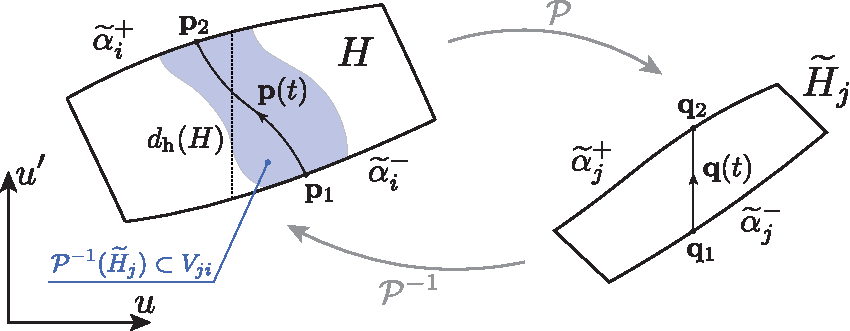
\includegraphics[scale = 1]{pic/thickness of h-strip (a)}
		\caption{
			Illustration to the proof of the point (ii) for the case when both h-strips $H$ and $\widetilde{H}_j$ and well-measurable.
			Thickness of $H$ is measured along the vertical dotted line, thickness of $\widetilde{H}_j$ is measured along the vertical line $\vb{q}(t)$.
			Arrows indicate the direction of motion along the curves while $t$ changes from $0$ to $1$.
			Pre-image of $\widetilde{H}_j$ strip is colored gray.
		}
	\label{fig:thickness-of-h-strip-a}
	\end{figure}
	
	Consider tangent vectors to $\vb{p}(t)$ and $\vb{q}(t)$ (upper dot means the derivative with respect to $t$):
	\begin{eqnarray}
		&& \dot{\vb{p}}(t) = (\dot{\psi}(t), \dot{\psi}'(t)); \\
		&& \dot{\vb{q}}(t) = (0, \dot{\phi}'(t)).
	\end{eqnarray}
	In each point $t$ they are connected by the $D \mathcal{P}_{\vb{p}(t)}$ operator
	\begin{equation}
		\dot{\vb{q}}(t) = D \mathcal{P}_{\vb{p}(t)} (\dot{\vb{p}}(t)).
	\end{equation}
	Rewrite this relation in a matrix form:
	\begin{equation}
		\begin{pmatrix}
			a_{11}(t) & a_{12}(t) \\ a_{21}(t) & a_{22}(t)
		\end{pmatrix}
		\begin{pmatrix}
			\dot{\psi}(t) \\
			\dot{\psi}'(t)
		\end{pmatrix} =
		\begin{pmatrix}
			0 \\ \dot{\phi}'(t)
		\end{pmatrix}.
	\end{equation}
	% TODO: Give a cite, from where follows this fact for Poincar\'e map.
	We take into account that matrix $(a_{mn})$ is a linearization of Poincar\'e map therefore its determinant $a_{11}(t) a_{22}(t) - a_{12}(t) a_{21}(t) = 1$ in each point $t$.
	From the relations above and the conditions of theorem on values of $a_{11}(t)$ it follows that
	\begin{equation}
		\dot{\phi}'(t) = \dfrac{1}{a_{11}(t)} \dot{\psi}'(t) \le \dfrac{1}{\mu} \dot{\psi}'(t).
	\label{eq:to-integrate}
	\end{equation}
	Integration of \eqref{eq:to-integrate} with limits $0 \le t \le 1$ gives:
	\begin{equation}
		d_{\mathrm{h}}(\widetilde{H}_j) = \phi_2' - \phi_1' = \int \limits_0^1 \dot{\phi}'(t) dt \le \dfrac{1}{\mu} \int \limits_0^1 \dot{\psi}'(t) dt = \dfrac{1}{\mu} (\psi_2' - \psi_1').
	\label{eq:thickness-of-strip-final}
	\end{equation}
	Curve $\vb{p}(t)$ is decreasing and boundaries of $H$ are increasing curves, so it follows from geometric considerations that $\psi_2' - \psi_1' \le d_{\mathrm{h}}(H)$, i.e. $d_{\mathrm{h}}(\widetilde{H}_j) \le (1 / \mu) d_{\mathrm{h}}(H)$.
	That gives the final statement of the theorem for well-measurable strips.
	
	\begin{figure}[h]
	\centering
		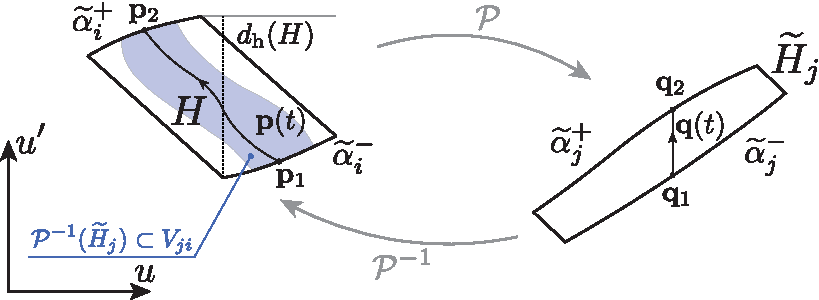
\includegraphics[scale = 1]{pic/thickness of h-strip (b)}
		\caption{
			Illustration to the proof of the point (ii) for the case when h-strip $H$ is not well-measurable.
			Its thickness is measured along the vertical dotted line.
			One endpoint of that line does not belong to the strip boundary $\widetilde{\alpha}_i^+$.
			Pre-image of $\widetilde{H}_j$ strip is colored with gray.
		}
	\label{fig:thickness-of-h-strip-b}
	\end{figure}
	
	The proof above can be easily generalized to the cases when h-strips  $H$ and $\widetilde{H}_j$ are not well-measurable.
	If strip $H$ is not well-measurable, the inequality $\psi_2' - \psi_1' \le d_{\mathrm{h}}(H)$ in \eqref{eq:thickness-of-strip-final} takes place also.
	This fact is illustrated on Figure~\ref{fig:thickness-of-h-strip-b}.
	Vertical distance between points $\vb{p}_1, \, \vb{p}_2$ turns out to be certainly less than the width of $H$ strip.
	
	In the case when h-strip $\widetilde{H}_j$ is not well-measurable, one should choose corner points $\vb{q}_1, \, \vb{q}_2$ in a such way that the vertical distance between them is equal to the thickness of $\widetilde{H}_j$, and then connect $\vb{q}_1, \, \vb{q}_2$ with a monotonic decreasing curve $\vb{q}(t)$, see Fig.~\ref{fig:thickness-of-h-strip-c}.
	This is always possible due to the geometric properties of not well-measurable h-strip.
	According to the choice of points $\vb{q}_1, \, \vb{q}_2$, $d_{\mathrm{h}}(\widetilde{H}_j) = \phi_2 - \phi_1$, and all the steps above remain valid since the corresponding cones mapping with all the consequences can be also applied for the decreasing curves $\vb{p}(t)$ and $\vb{q}(t)$.
	\begin{figure}[h]
	\centering
		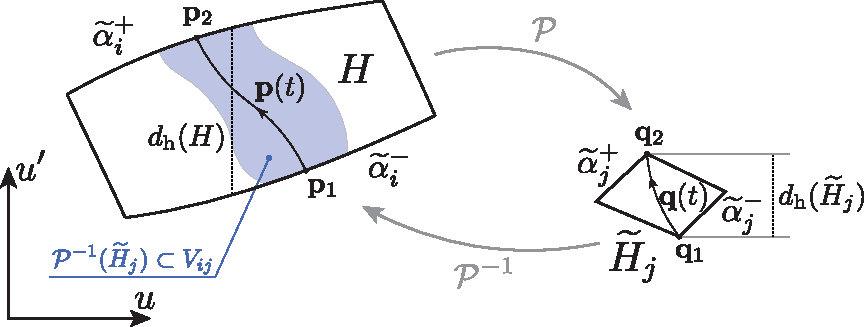
\includegraphics[scale = 1]{pic/thickness of h-strip (c)}
		\caption{
			Illustration to the proof of the point (ii) for the case when h-strip $\widetilde{H}_j$ is not well-measurable.
			Thickness of $H$ and $\widetilde{H}_j$ are measured along the dotted lines.
			Pre-image of $\widetilde{H}_j$ strip is colored with gray.
	  }
	\label{fig:thickness-of-h-strip-c}
	\end{figure}
	
	If both h-strips $H$ and $\widetilde{H}_j$ are not well-measurable then the two above mentioned technics should be combined together.
	The consideration of all other cases of the theorem is similar and the same reasoning can be applied with minor adjustments.
	Theorem is proved.
\end{proof}

\pagebreak

\begin{theorem}[On v-strips mapping]
\label{thm:v-strips-mapping}
	Let Poincar\'e map $\mathcal{P}$ and its inverse $\mathcal{P}^{-1}$ be defined on a complete (see Definition~\ref{def:complete-island-set}) island set $\bigcup_{i \in S} D_i$, where $S$ is a finite or countable set of indices.
	Let for all $i, j \in S$ the set $H_{ij} = \mathcal{P} (D_i) \cap D_j$ is non-empty, $\mathcal{P}^{-1}$ is defined on a
	 closure $\overline{H_{ij}}$, and one of the following two conditions holds:
	\begin{enumerate}
		\item[(1)] the borders $\beta_j^{\pm}$ of an island $D_j$ are increasing curves, $\forall \vb{q} \in \overline{H_{ij}}$ the signs of $\{ b_{mn} \}$ in the matrix of the linear operator $D \mathcal{P}_{\vb{q}}^{-1} = (b_{mn})$ have exactly one of the following configurations:
			\begin{center}
				(a) $\begin{psm} + & + \\ + & + \end{psm}$, \quad
				(b) $\begin{psm} - & - \\ - & - \end{psm}$, \quad
				(c) $\begin{psm} + & + \\ - & - \end{psm}$, \quad
				(d) $\begin{psm} - & - \\ + & + \end{psm}$;
			\end{center}
			and at the same time the borders $\beta_i^{\pm}$ of $D_i$ are increasing curves for cases (a), (b), and decreasing curves for (c), (d);
		\item[(2)] the borders $\beta_j^{\pm}$ of an island $D_j$ are decreasing curves, $\forall \vb{q} \in \overline{H	_{ij}}$ the signs of $\{ b_{mn} \}$ in the matrix of the linear operator $D \mathcal{P}_{\vb{q}}^{-1} = (b_{mn})$ have exactly one of the following configurations:
			\begin{center}
				(a) $\begin{psm} + & - \\ - & + \end{psm}$, \quad
				(b) $\begin{psm} - & + \\ + & - \end{psm}$,	\quad
				(c) $\begin{psm} + & - \\ + & - \end{psm}$, \quad
				(d) $\begin{psm} - & + \\ - & + \end{psm}$;		
			\end{center}
			and at the same time borders $\beta_i^{\pm}$ of $D_i$ are decreasing curves for cases (a), (b), and increasing for (c), (d);
	\end{enumerate}
	and moreover $\exists \nu > 1$ such that $\forall q \in \overline{H_{ij}}$, $|b_{22}| \ge \nu$.
	Then
	\begin{itemize}
		\item[(i)] for any \emph{v}-strip $V \in D_j$, $\mathcal{P}^{-1} (V) \cap D_i = \widetilde{V}_i$ is also a \emph{v}-strip;
		\item[(ii)] $d_{\mathrm{v}} (\widetilde{V}_i) \le (1 / \nu) d_{\mathrm{v}} (V)$ (here $d_{\mathrm{v}}(\cdot)$ is an \emph{v}-strip thickness in a sence of Definition~\ref{def:v-thickness}).
	\end{itemize}
\end{theorem}
\begin{proof}
	Completely analogous to the proof of the h-strips mapping theorem.
\end{proof}